%   Filename    : chapter_3.tex 
\chapter{Research Methodology}
\label{sec:methodology}

This chapter discusses the materials and methods to be employed in the study, focusing on the development requirements and the software, and languages utilized. This will also entail the overall workflow in conducting the study, Non-Invasive Methods in Determining the Sex of \textit{Tegillarca granosa} (blood cockles) using machine learning technologies. The different machine and deep learning and computer vision technologies will be thoroughly discussed to ensure a comprehensive understanding of the entity of the research endeavor and its processes. 

Dr. Victor Emmanuel Ferriols, the director of the Institute of Aquaculture, will oversee the overall workflow and conduct of this experiment. The researchers will also be guided by the research associates, LC Mae Gasit and Allena Esther Artera. Consequently, the whole dataset collection process will be done at the University of the Philippines Visayas hatchery facility. 

The methodology is consists of ten parts: (1) Sample Collection, (2) Ethical Considerations, (3) Creating \textit{T.granosa} Dataset, (4) Morphological Characteristics Collection (5) Image Acquisition and Pre-processing, (6) Hardware and Software Configuration, (7) Data Augmentation (8) Machine and Deep Learning Technologies, (9) Machine Learning Models for Pre-evaluation, and (10) Deep Learning for Image-Based Classification. 

\section{Sample Collection}
\label{sec:samplecollect}
The collection of \Tgranosa samples used in this study is part of an ongoing research project by the UPV DOST-PCAARRD titled "Establishment of the Center for Mollusc Research and Development: Development of Spawning and Hatchery Techniques for the Blood Cockle (\textit{Anadara granosa}) for Sustainable Aquaculture." This research project provides a total of 500 adult \textit{T. granosa} samples which undergo spawning and are classified by sex as either male or female. The samples, ranging in size from 34 to 61 mm, are sourced from the coastal area of Zaraga, Iloilo, Philippines and fish markets in Ivisan, Capiz, Philippines. 

The research and experimentation take place at the University of the Philippines Visayas hatchery facility in Miagao, Iloilo, Philippines, where the samples are maintained in 200 L fiberglass reinforced plastic (FRP) tanks containing filtered seawater with 35 ppt salinity \cite{miranda2023}. 

Spawning is induced through temperature fluctuations which is the most natural and least invasive method for bivalves compared to other methods \cite{aji}. However, due to a shortage of female spawned samples, additional blood cockles were dissected. This dissection process is carried out personally by the researchers, assisted by hatchery staff. The sex of the dissected samples is identified based on the coloration of the gonad tissue, which varies by sex and maturity stage. Females exhibit orange-red to pale orange gonads while males display white to grayish-white gonads \cite{may2021}.

\begin{figure}[!htbp]
	\centering
	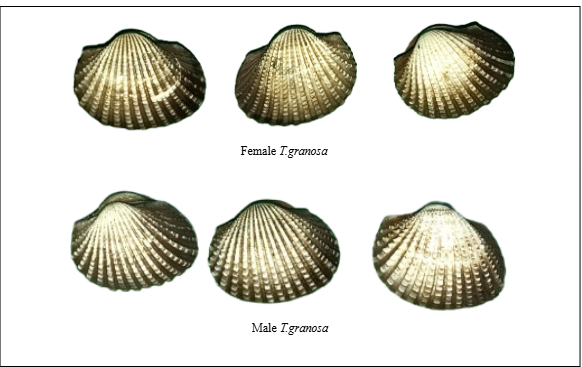
\includegraphics[width=0.9\textwidth]{figures/male-female T.granosa.png}
	\caption{Male and Female \Tegillarcagranosa shells}
\end{figure}

\section{Ethical Considerations}
\label{sec:ethical}

This study did not require ethical approval for working with animals, as per local legislation and institutional guidelines, since the experiments were performed on species commonly consumed as food by humans.


\section{Creating \textit{T. granosa} Dataset}
\label{sec:dataset}

For the initial preparation of the experiment, the researchers will collect primary observations for 100 samples of \textit{T. granosa.}. For the actual experimentation, the researchers will collect the original dataset by batch eventually comprising 500 samples of \textit{T. granosa}. The linear measurements were measured and gathered manually by the researchers and compiled in the CSV file separating male and female \textit{T. granosa}. 

On the other hand, the images captured for the dataset will be saved in jpg format with a file naming convention of the sample’s sex, the orientation or view of the shell, and its corresponding number out of the total 500 samples. Female \textit{T. granosa} samples will begin with 0 in their file name, while males will begin with 1, followed by the views captured such as (1) dorsal, (2) ventral, (3) anterior, (4) posterior, (5) left lateral, and (6) right lateral (refer to Figure~\ref{fig:granosa_views}), and lastly, a unique sample number. For example, “010001” will be the file name for the first female sample taken from the dorsal view, and “110001” for the first male sample also taken from the dorsal view. 

The dataset will be organized in a CSV file that lists each image’s file name along with their shell’s width, height, length, rib count, length of the hinge line, and distance between their umbos. This dataset will be essential for machine learning model training and testing. 

\begin{figure}[!htbp]
	\centering
	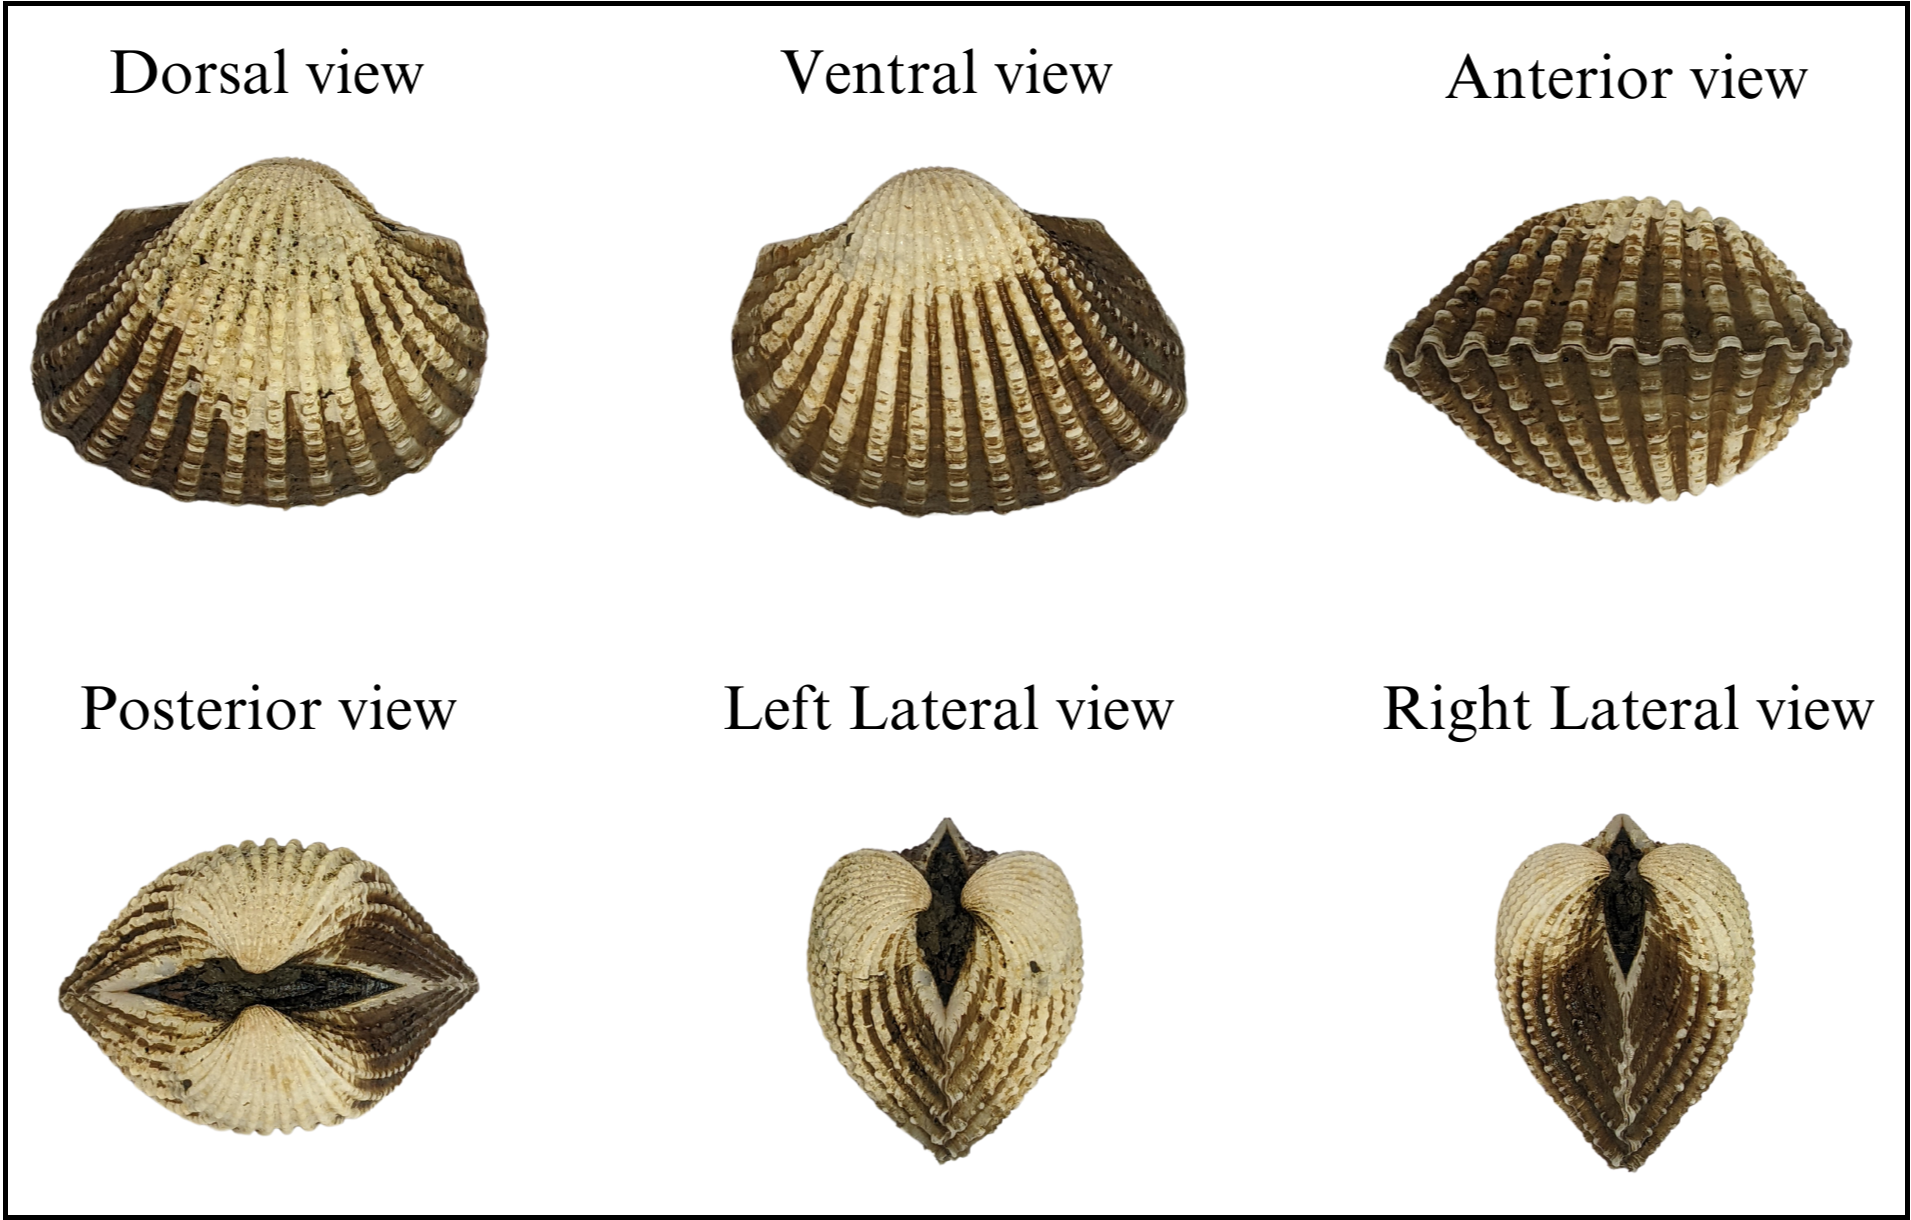
\includegraphics[width=0.9\textwidth]{figures/view.png}
	\caption{Different Views of the \textit{T. granosa} Shell Captured}
	\label{fig:granosa_views}
\end{figure}

\newpage
\section{Morphological and Morphometric Characteristics Collection}
\label{sec:morphochar}

Morphology refers to the biological form and represents one of the most visually recognizable phenotypes across all organisms \cite{tsutsumi2023}. Morphology is a term that describes structural characteristics by measuring specific components, namely, dimensions such as shapes, sizes, and colors. As stated by the researchers, quantifying and characterizing the shape is essential to understanding and visualizing the variations in \textit{T. granosa’s} morphology. 

In this study, the researchers are going to measure the height, width, and length of \textit{T. granosa.} The dimensions will be recorded using a Vernier caliper to the nearest 0.01 mm. For the measurements, refer to Figure~\ref{fig:linear_measurements}. The length (A) of the \textit{T. granosa} refers to the measurement from the anterior to the posterior of the shell. The width (B) is measured through the shell’s widest point from the left to the right valve. The height (C) is measured from the base of the shell to the shell’s apex. The height of the gap between the valves (C) near the hinge will also be measured for the length of the hinge line and the distance between the umbos. The authors, Reyment and Kennedy (1998), indicated that the use of counts of the shell ribs as supplementary information increases identification accuracy. Thus, the researchers will also take into account the difference in the rib count of the male and female \textit{T. granosa}, and the ratio will be calculated since the sizes of the blood cockles vary. Sex ratio, size frequency distribution, and relative growth rates will be used to investigate sexual dimorphism.

\begin{figure}[!htbp]
	\centering
	\includegraphics[width=0.95\textwidth]{figures/Tegillarca_granosa_linear_measurements.png}
	\caption{Linear Measurements of  \Tegillarcagranosa shell.}
	\label{fig:linear_measurements}
\end{figure}

\section{Image Acquisition and Pre-Processing}
\label{sec:imageprocess}
In this study, an original dataset of \textit{Tegillarca granosa} will be built with 500 images (250 male blood cockles images and 250 female images). Both the male and female \Tgranosa images will contain 1500 images from different angles. During the data gathering process, there seemed to be an unbalanced number of spawned samples in favor with the male blood cockles. Thus, this can cause the data to be unbalanced. Unbalanced samples will lead to train model slowly and affect the gradient update. So, the dataset needs to meet sample equilibrium criteria \cite{cui2020}. The researchers constructed a controlled environment for capturing the images of the samples utilizing a box-like structure with a white background surface. This setup was designed to maintain uniform captures of the images, and a consistent measurement between the sample and the camera, fixing the camera at a consistent angle above the \textit{T. granosa}. To ensure the image quality, eliminate shadows, and clarity of the sample during the image acquisition process, the ring light will be placed in front of the box and use a camera without flash. Google Pixel 3 XL is the smartphone that will be utilized with the following specifications: 2960 x 1440 for the resolution, 4,032 x 3,024 pixels (12.2 MP) for the dimensions, f/1.8 for the fstop, 28mm (wide), ½.55”, 1.4µm, dual pixel PDAF, OIS \cite{concepcion2023}

\begin{figure}[!htbp]
	\centering
	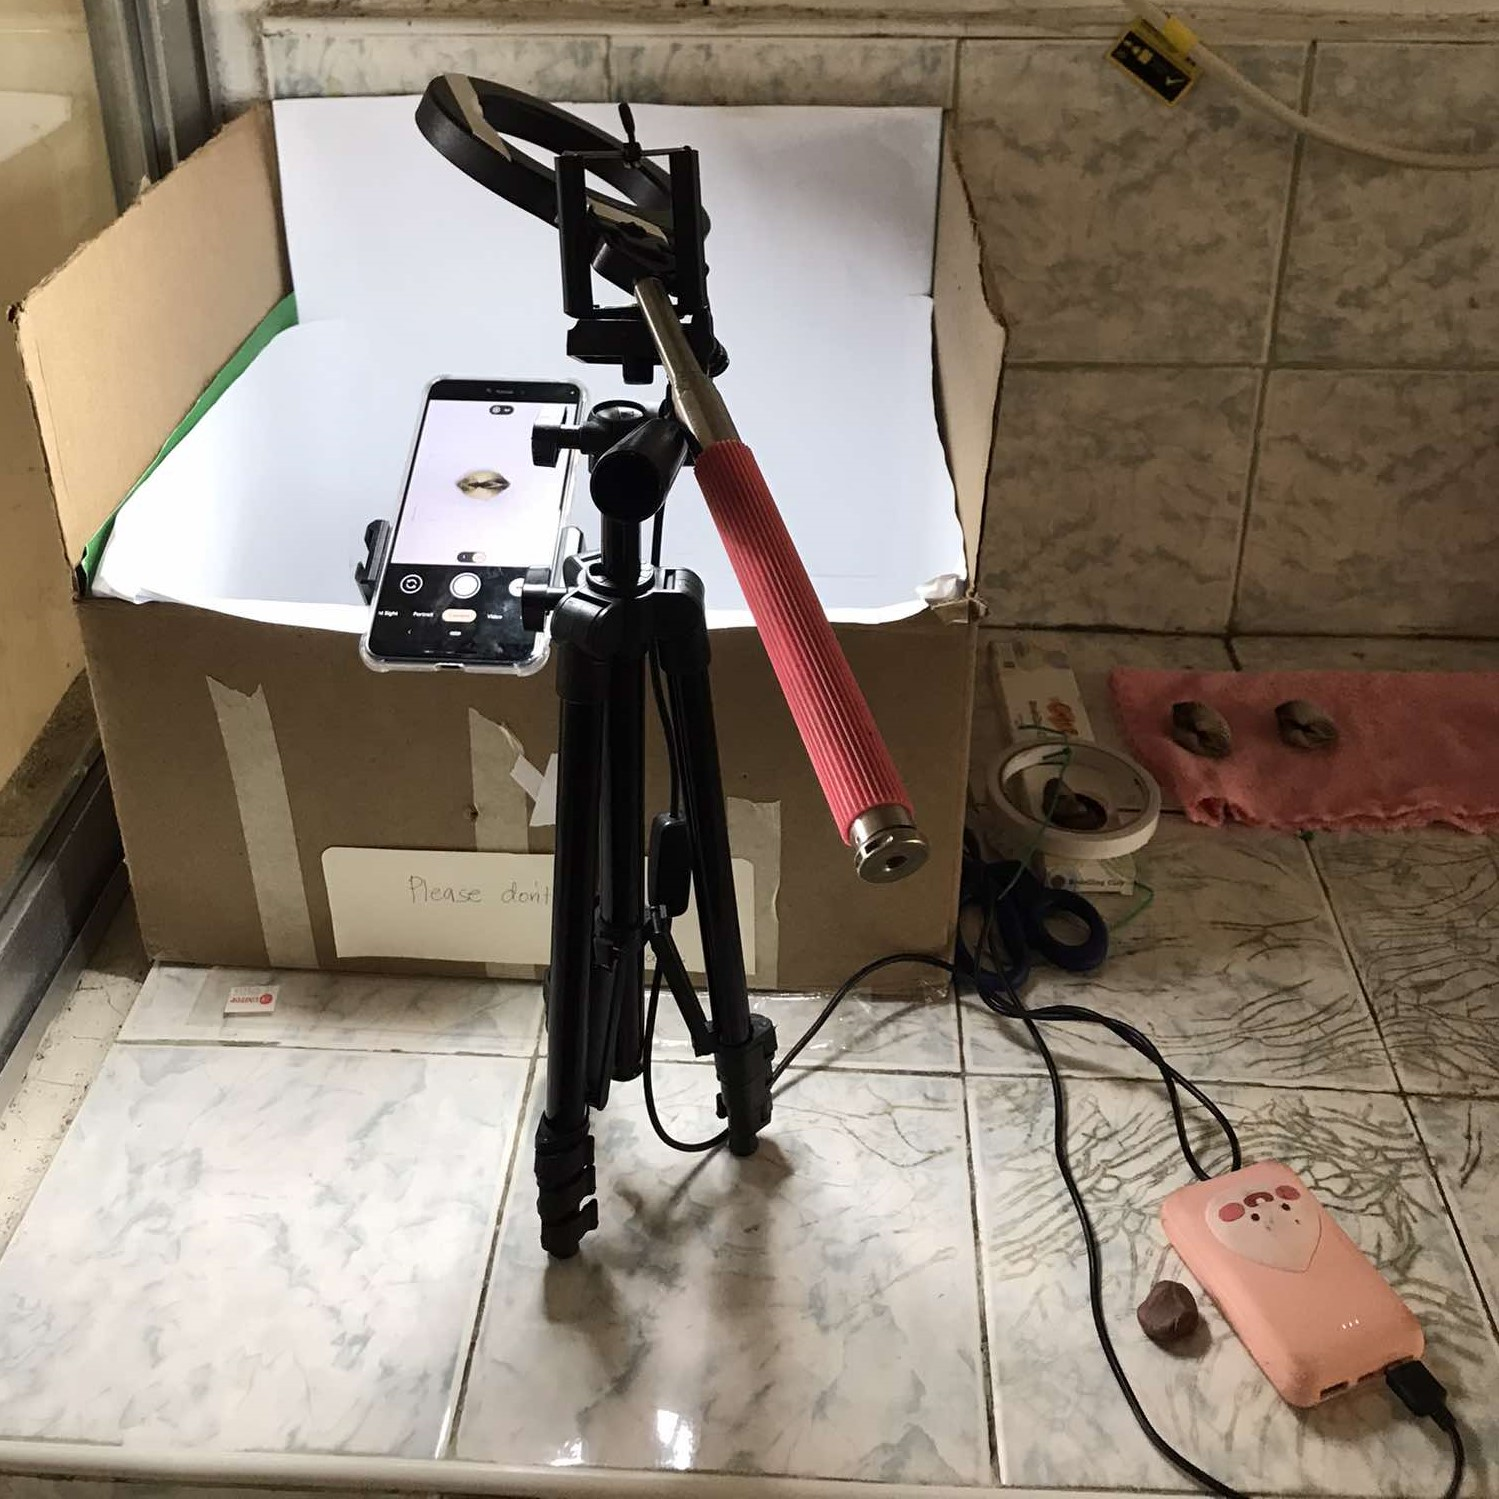
\includegraphics[width=0.4\textwidth]{figures/setup.jpg}
	\caption{Image Acquisition Setup for \textit{T. granosa} Samples}
	\label{fig: setup}
\end{figure}

\section{Hardware and Software Configuration}
The machine learning and deep learning algorithms would be trained on ACER Aspire 3 general processing unit (GPU) which has a central processing unit (CPU) of  AMD Ryzen 3 7320U with Radeon Graphics (8) @ 2.395GHz and with a memory of 8 gigabytes (GB). The model will be performed on Keras which is a deep learning framework integrated with TensorFlow \cite{cui2020}.

\section{Data Augmentation}
In the practice of deep learning, there is a possibility of a small dataset to being filled with bias and overfitting. The most obvious solution is to add more samples however, it is time-consuming and labor-intensive to collect a massive amount of data. In dealing with an unbalanced dataset, various data augmentation techniques can be used, such as rotation, scaling, shearing, and translation. These four data augmentation technique will be applied to generate 10 new images for each image. \cite{cui2020}. Thus, from a total of 3000 images, where 6 angles are captured for each of the 500 samples, it would enlarge to 120,000 images that will be used in training the state-of-the-art CNN models. 

\section{Machine and Deep Learning Technologies}

This section of the paper will discuss the technologies to be used in training, and testing the model as well as associated techniques and algorithms. Since obtaining the induced samples will be done per batch, the researchers will conduct an initial run with supervised machine learning models to determine the significance of the collected linear measurements (length, width, height, length hinge line, distance between umbos, and rib count) before delving into more complex methods such as deep learning CNN models. 

\section{Morphometric Characteristics Evaluation using Machine Learning }
\label{sec:ml models}

The shape of recording structures was first analyzed by collecting measurements of linear distances and applying multivariate statistical methods to these data (traditional linear measurement method) \cite{rohlf1984}. Geometric morphometric (GM) methods are an alternative way of analyzing and quantifying shape, which in theory retains more detail about the geometry of the structure than could be obtained from linear measurements \cite{adams2004}. Machine learning techniques such as decision tree classification, support vector machines (SVMs), and k-nearest neighbors (KNN) have been applied to the analysis of bivalve shell geometry and morphology to classify shells based on morphological features, including shell shape, size, and texture, among others \cite{kiel2021}. The results of these studies have shown that machine learning algorithms can accurately classify bivalve shells and provide insights into the relationships between shell morphology and various environmental factors.
Following this, the researchers are going to conduct a pre-evaluation of the linear measurements for 100 samples of \textit{T. granosa} using a Support Vector Machine in order to determine whether these measurements can serve as a reliable factor in determining the sex of the samples before proceeding to more complex methods. 

\subsection{Extreme Gradient Boosting}
Extreme Gradient Boosting (XGBoost) is a DT-based ensemble machine learning algorithm that combines the gradient boosting framework and decision trees to reach a final decision. It has the ability to achieve improved performance and higher accuracy compared to other supervised machine learning models. This model would be beneficial in terms of its key capabilities of computation of the importance of the attributes based on the overall contribution to the accuracy of the predictions \cite{torres2023}. 

\subsection{Logistic Regression}

Logistic Regresion (LR) is the process of modeling the probability of a discrete outcome given the input variable. The outcomes in the logistic regression is measured using a binary variable and is a transformation of the linear regression using the sigmoid function \cite{cui2020}. Although there are no related studies about sex identification in mollusks, logistic regression is a useful analysis method in classification problems such as determining the sexual dimorphism given the linear measurements measured. 

\subsection{Random Forest}

Random Forest (RF) is a type of supervised machine learning algorithm that is often used in regression and classification problems \cite{cui2020}. It has also been utilized in mollusks studies such as sex identification of abalone wherein the Random Forest achieved the highest average balance accuracy for all the datasets \cite{arifin2021}.

\subsection{Support Vector Machine}

Support Vector Machine (SVM) is a supervised machine learning algorithm that classifies data by finding the optimal hyperplane which is also used in classification and regression problems \cite{cui2020}. Support vector machine is also widely used in aquaculture related studies such as the sex determining mandible shapes due to its ability to solve classification problems with high validation accuracy especially when the clusters of the data with varying labels. The SVM has the ability to reflect the degree of cluster separation. It has the ability to be used as a tool in the variety of the image data with biological shapes \cite{tsutsumi2023}.

\subsection{k-Nearest Neighbors}
The k-Nearest Neighbor (KNN) algorithm is a method commonly used for regression and classification tasks. It was applied in the study "Identification of Asian Green Mussel \textit{Perna Viridis}' Sex Using Image Processing, Fuzzy Logic, and K-Nearest Neighbor," where KNN achieved 100\% accuracy in classifying the sex of 50 male and 50 female mussels during the initial training phase with a dataset of 100 samples \cite{magbayao2020}.

\section{ Deep Learning for Image-Based Classification}
\label{sec:deeplearning}
After collecting a sufficient number of images and identifying initial patterns, convolutional neural networks (CNNs) will be used. CNNs, models like VGGNet, Inception ResNet, and SqueezeNet have been effectively applied in phenotype classification \cite{kim2024}. In this study, the deep learning model will be specifically adapted for the sex identification of \textit{T. granosa} based on shell images. CNN has achieved breakthroughs in terms of image classification, image segmentation, and speech recognition \cite{he2018}. In this study, CNNs will analyze the images and learn important details about their shapes that can help identify whether they are male or female. Due to the limitation of literature focusing on the sex determining mechanism for bivalves, particularly \textit{T. granosa}, the researchers will implement and compare three of the state-of-thea-art CNN models namely VGGNet, Inception ResNet, and Squeezenet \citeA{kim2024}. 

\subsection{CNN Model: Visual Geometry Group}
Visual Geometry Group (VGG) is considered to be a standard Convolutional Neural Network (CNN) architecture that is comprised of multiple layers that has been a ground-breaking object detection models and one of the most popular image recognition architecture \cite{boesch2021}. 

\subsection{CNN Model: Inception ResNet}
Inception ResNet is a convolutional neural network that has been trained on more than a million images and has 164 deep layers that have the capacity to classify varied images \cite{mathworks}. This model is mainly used in bivalve studies such as in identifying different ark shells \cite{kim2024}.  

\subsection{CNN Model: SqueezeNet}
SqueezeNet is particularly advantageous because it reduces the number of parameters and amount of memory required to store the model without sacrificing accuracy \cite{koonce2021}. Its ability to achieve high accuracy in classifying shell images makes it a suitable choice for distinguishing between male and female \textit{T. granosa.}

\section{Evaluation Metrics for Machine Learning and CNN Models}
Evaluating the performance of the binary classification model is important as well as selecting the appropriate metrics that is based on the requirements of the user. The performance of the supervised machine learning models will be measured based on three metrics namely: accuracy, precision, recall, and F1 score. 

Accuracy (ACC) is the ratio of the overall correctly predicted samples to the total number of examples in the evaluation dataset \cite{cui2020}. The overall correctness of the model in predicting male and female blood cockles. This metric could help in understanding how well the model performs across all classifications. The formula for the accuracy is: 

\begin{equation}
	\text{PREC} = \frac{\text{Correctly classified samples}} {\text{All samples }} = \frac{TP+ TN}{TP + FP + TN + FN}
	\label{eq:acc}
\end{equation}
Precision (PREC) is the ratio between correctly predicted samples in all samples that are assigned to the positive class \cite{cui2020}. This metric promotes fair representation and prevents the misidentification of blood cockles as it identifies potential inaccuracies or biases. The formula for precision is:


\begin{equation}
	\text{PREC} = \frac{\text{True positive samples}} {\text{Samples assigned to class }} = \frac{TP}{TP + FP}
	\label{eq:prec}
\end{equation}

Recall (REC) is known as the sensitivity or the true positive rate (TPR) which is the ratio of the correctly predicted cases from all the samples assigned to the actual positive cases \cite{cui2020}. This metric is the ability of the model to correctly identify positive male and female samples. The formula for the recall is:

\begin{equation}
	\text{REC} = \frac{\text{True positive samples}} {\text{Samples classified positive}} = \frac{TP}{TP + FN}
	\label{eq:rec}
\end{equation}

F1 score (F1) is defined as the mean of the precision and recall in which it penalizes the extreme values of either of the two \cite{cui2020}. The formula for the F1 is: 

\begin{equation}
	\text{REC} = \frac{ precision \times recall }{precision \times recall }= \frac{2 \times TP}{2 \times TP + FP + FN}
	\label{eq:f1}
\end{equation}
